%%%%%%%%%%%%%%%%%%%%%%%%%%%%%%%%%%%%%%%%%%%%%%%%%%%%%%%%%%%%%%%%%%%%%%
%%%%                   Compartment
%%%%%%%%%%%%%%%%%%%%%%%%%%%%%%%%%%%%%%%%%%%%%%%%%%%%%%%%%%%%%%%%%%%%%%

\section{Glyph: \glyph{Compartment}}\label{sec:compartment}

A compartment is a logical or physical structure that contains entity pool nodes. An \glyph{EPN} can only belong to one compartment. Therefore, the ``same'' biochemical species located in two different compartments are in fact two different ``pools'' and should be represented by two \glyph{EPNs}.  A compartment is represented by a surface enclosed in a continuous border or located between continuous borders. These borders should be noticeably thicker than the borders of the \glyph{EPNs}. A compartment can take \textbf{any} geometry. A compartment must always be entirely enclosed.

\begin{figure}[H]
  \centering
  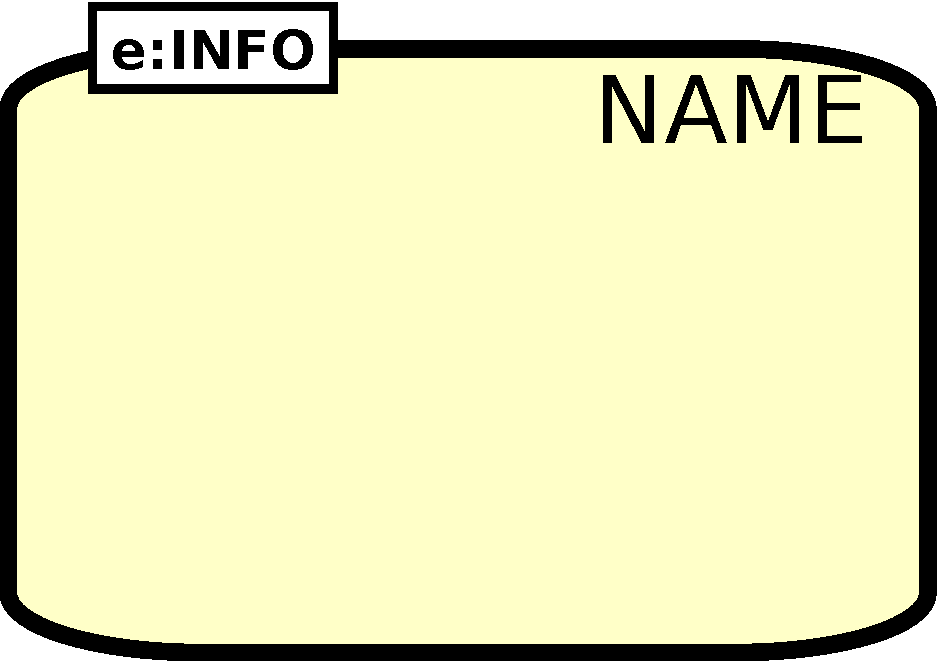
\includegraphics[scale = 0.3]{images/compartment}
  \caption{The \PD glyph for \glyph{compartment}.}
  \label{fig:compartment}
\end{figure}

To allow more aesthetically pleasing and understandable maps, compartments are allowed to overlap each other visually, but it must be kept in mind that this does not mean the top compartment contains part of the bottom compartment. 